
%%%%%%%%%%%%%%%%%%%%%%%%%%%%%%%%%%%%%%%%%%%%%%%%%%%%%%%%%%%%%%%%%%%%%
%% This is a (brief) model paper using the achemso class
%% The document class accepts keyval options, which should include
%% the target journal and optionally the manuscript type.
%%%%%%%%%%%%%%%%%%%%%%%%%%%%%%%%%%%%%%%%%%%%%%%%%%%%%%%%%%%%%%%%%%%%%
\documentclass[journal=jacsat,manuscript=article]{achemso}

%%%%%%%%%%%%%%%%%%%%%%%%%%%%%%%%%%%%%%%%%%%%%%%%%%%%%%%%%%%%%%%%%%%%%
%% Place any additional packages needed here.  Only include packages
%% which are essential, to avoid problems later. Do NOT use any
%% packages which require e-TeX (for example etoolbox): the e-TeX
%% extensions are not currently available on the ACS conversion
%% servers.
%%%%%%%%%%%%%%%%%%%%%%%%%%%%%%%%%%%%%%%%%%%%%%%%%%%%%%%%%%%%%%%%%%%%%
\usepackage[version=3]{mhchem} % Formula subscripts using \ce{}

%%%%%%%%%%%%%%%%%%%%%%%%%%%%%%%%%%%%%%%%%%%%%%%%%%%%%%%%%%%%%%%%%%%%%
%% If issues arise when submitting your manuscript, you may want to
%% un-comment the next line.  This provides information on the
%% version of every file you have used.
%%%%%%%%%%%%%%%%%%%%%%%%%%%%%%%%%%%%%%%%%%%%%%%%%%%%%%%%%%%%%%%%%%%%%
%%\listfiles

%%%%%%%%%%%%%%%%%%%%%%%%%%%%%%%%%%%%%%%%%%%%%%%%%%%%%%%%%%%%%%%%%%%%%
%% Place any additional macros here.  Please use \newcommand* where
%% possible, and avoid layout-changing macros (which are not used
%% when typesetting).
%%%%%%%%%%%%%%%%%%%%%%%%%%%%%%%%%%%%%%%%%%%%%%%%%%%%%%%%%%%%%%%%%%%%%
\newcommand*\mycommand[1]{\texttt{\emph{#1}}}

%%%%%%%%%%%%%%%%%%%%%%%%%%%%%%%%%%%%%%%%%%%%%%%%%%%%%%%%%%%%%%%%%%%%%
%% Meta-data block
%% ---------------
%% Each author should be given as a separate \author command.
%%
%% Corresponding authors should have an e-mail given after the author
%% name as an \email command. Phone and fax numbers can be given
%% using \phone and \fax, respectively; this information is optional.
%%
%% The affiliation of authors is given after the authors; each
%% \affiliation command applies to all preceding authors not already
%% assigned an affiliation.
%%
%% The affiliation takes an option argument for the short name.  This
%% will typically be something like "University of Somewhere".
%%
%% The \altaffiliation macro should be used for new address, etc.
%% On the other hand, \alsoaffiliation is used on a per author basis
%% when authors are associated with multiple institutions.
%%%%%%%%%%%%%%%%%%%%%%%%%%%%%%%%%%%%%%%%%%%%%%%%%%%%%%%%%%%%%%%%%%%%%
\author{Hongjian Li}
\email{jackyleehongjian@gmail.com}
\author{Kwong-Sak Leung}
\author{Man-Hon Wong}
\affiliation[Chinese University of Hong Kong]
{Department of Computer Science and Engineering, Chinese University of Hong Kong, Shatin, New Territories, Hong Kong}
\author{Pedro J. Ballester}
\email{pedro.ballester@ebi.ac.uk}
\affiliation[European Bioinformatics Institute]
{European Bioinformatics Institute, Wellcome Trust Genome Campus, Hinxton, Cambridge - CB10 1SD, UK}

%%%%%%%%%%%%%%%%%%%%%%%%%%%%%%%%%%%%%%%%%%%%%%%%%%%%%%%%%%%%%%%%%%%%%
%% The document title should be given as usual. Some journals require
%% a running title from the author: this should be supplied as an
%% optional argument to \title.
%%%%%%%%%%%%%%%%%%%%%%%%%%%%%%%%%%%%%%%%%%%%%%%%%%%%%%%%%%%%%%%%%%%%%
\title[RF::Cyscore]{Improving Protein-Ligand Binding Affinity Prediction by Substituting Random Forest for Multiple Linear Regression: Using Cyscore as an Example}

%%%%%%%%%%%%%%%%%%%%%%%%%%%%%%%%%%%%%%%%%%%%%%%%%%%%%%%%%%%%%%%%%%%%%
%% Some journals require a list of abbreviations or keywords to be
%% supplied. These should be set up here, and will be printed after
%% the title and author information, if needed.
%%%%%%%%%%%%%%%%%%%%%%%%%%%%%%%%%%%%%%%%%%%%%%%%%%%%%%%%%%%%%%%%%%%%%
\abbreviations{MLR,RF}
\keywords{Molecular docking, binding affinity, machine learning}

%%%%%%%%%%%%%%%%%%%%%%%%%%%%%%%%%%%%%%%%%%%%%%%%%%%%%%%%%%%%%%%%%%%%%
%% The manuscript does not need to include \maketitle, which is
%% executed automatically.
%%%%%%%%%%%%%%%%%%%%%%%%%%%%%%%%%%%%%%%%%%%%%%%%%%%%%%%%%%%%%%%%%%%%%
\begin{document}

%%%%%%%%%%%%%%%%%%%%%%%%%%%%%%%%%%%%%%%%%%%%%%%%%%%%%%%%%%%%%%%%%%%%%
%% The "tocentry" environment can be used to create an entry for the
%% graphical table of contents. It is given here as some journals
%% require that it is printed as part of the abstract page. It will
%% be automatically moved as appropriate.
%%%%%%%%%%%%%%%%%%%%%%%%%%%%%%%%%%%%%%%%%%%%%%%%%%%%%%%%%%%%%%%%%%%%%
\begin{tocentry}

Some journals require a graphical entry for the Table of Contents.
This should be laid out ``print ready'' so that the sizing of the
text is correct.

Inside the \texttt{tocentry} environment, the font used is Helvetica
8\,pt, as required by \emph{Journal of the American Chemical
Society}.

The surrounding frame is 9\,cm by 3.5\,cm, which is the maximum
permitted for  \emph{Journal of the American Chemical Society}
graphical table of content entries. The box will not resize if the
content is too big: instead it will overflow the edge of the box.

This box and the associated title will always be printed on a
separate page at the end of the document.

\end{tocentry}

%%%%%%%%%%%%%%%%%%%%%%%%%%%%%%%%%%%%%%%%%%%%%%%%%%%%%%%%%%%%%%%%%%%%%
%% The abstract environment will automatically gobble the contents
%% if an abstract is not used by the target journal.
%%%%%%%%%%%%%%%%%%%%%%%%%%%%%%%%%%%%%%%%%%%%%%%%%%%%%%%%%%%%%%%%%%%%%
\begin{abstract}

State-of-the-art protein-ligand docking methods are generally limited by the traditionally low accuracy of their scoring functions, which are used to predict binding affinity and thus vital for discriminating between active and inactive compounds. Despite intensive research in recent years, many newly-developed scoring functions hardly show satisfactory prediction performance. They often assume a predetermined additive functional form for some sophisticated numerical features, and utilize standard least-square multivariate linear regression on experimental data to derive the coefficients. In this study we show that such a simple functional form is detrimental for its performance, and replacing linear regression by machine learning techniques like random forest (RF) can significantly improve prediction performance. Most importantly, we investigate the conditions of applying RF and find that RF requires sufficient features and training samples to implicitly capture the non-linearity between structural features and measured binding affinities. Lastly, we show that RF-based scoring functions can be as interpretable as classical ones. We use Cyscore, an empirical scoring function recently published in a top journal, as baseline.

\end{abstract}

%%%%%%%%%%%%%%%%%%%%%%%%%%%%%%%%%%%%%%%%%%%%%%%%%%%%%%%%%%%%%%%%%%%%%
%% Start the main part of the manuscript here.
%%%%%%%%%%%%%%%%%%%%%%%%%%%%%%%%%%%%%%%%%%%%%%%%%%%%%%%%%%%%%%%%%%%%%
\section{Introduction}

Protein-ligand docking is a structural bioinformatic method that predicts how a ligand binds to a target protein and their binding affinity. Hence docking is useful in elaborating intermolecular interactions and enhancing the potency and selectivity of binding in subsequent phases of the modern drug discovery process. Docking has a wide variety of pragmatic and successful applications in structure-based virtual screening, drug repurposing, lead compound optimization, protein cavity identification, protein function prediction, etc.

Docking consists of two major operations: predicting the position, orientation and conformation of a ligand when docked to the protein's binding pocket, and predicting their binding strength. The former operation is known as pose generation, and the latter is known as scoring. State-of-the-art docking methods, such as AutoDock Vina \cite{595} and idock \cite{1153}, have managed to cope with the pose generation problem with a redocking success rate of over 50\% \cite{1362} on the benchmarks of both PDBbind v2012 and v2011 \cite{529,530} and the CSAR NRC HiQ Set 24Sept2010 \cite{857,960}. Therefore the single most critical limitation of docking is the traditionally low accuracy of the scoring functions.

Classical scoring functions assume a fixed functional form for the relationship between the numerical features that characterize the protein-ligand complex and its predicted binding affinity. Such functional form is typically inspired by some sorts of established chemistry theories, and is often additive. The overall binding affinity is calculated as a weighted sum of several physically meaningful terms, while their coefficients are typically derived from standard least-square multivariate linear regression (MLR) on experimental data. Cyscore \cite{1372}, a recently published empirical scoring function, is an example of classical scoring functions.

Cyscore assumes that the overall protein-ligand binding free energy can be decomposed into four terms: hydrophobic free energy, van der Waals interaction energy, hydrogen bond interaction energy and ligand's conformational entropy. Cyscore mainly focuses on improving the prediction of hydrophobic free energy by using a novel curvature-dependent surface-area model, which was claimed to be able to distinguish convex, planar and concave surface in hydrophobic free energy calculation.

In addition to classical scoring functions, recent years have seen a growing number of new developments of machine-learning scoring functions, with RF-Score \cite{564} being one of the representatives (see \cite{1373} for a comprehensive review). RF-Score, as its name suggests, uses Random Forest (RF) \cite{1309} to implicitly learn the functional form in an entirely data-driven manner, and thus circumvents the modelling assumption of classical scoring functions. RF-Score was shown to remarkably outperform 16 classical scoring functions when evaluated on the common PDBbind v2007 benchmark \cite{564}. Despite being a recent development, RF-Score has already been successfully used to discover a large number of innovative binders against antibacterial DHQase2 targets \cite{1281}. For the purpose of prospective virtual screening, RF-Score has now been incorporated into istar \cite{1362}, a user-friendly large-scale docking service available at http://istar.cse.cuhk.edu.hk/idock.

In this study we compare the prediction performance of two regression models MLR and RF, and investigate their application conditions under various contexts.

\section{Methods}

%This section introduces two regression models MLR and RF, three benchmarks to evaluate performance of the two regression models, and the performance metrics used in this study.

\subsection{Multiple Linear Regression (MLR)}

Cyscore is a classical empirical scoring function in an additive functional form of four terms (Eq. \ref{eqn:cyscore}), whose coefficients were obtained by MLR on 247 high-quality complexes carefully selected from PDBbind v2012 refined set. The intercept value was not reported in the original publication, but was included in this study in order to compute absolute binding affinity values.

\begin{equation}
\Delta G_{bind} = k_h\Delta G_{hydrophobic} + k_v\Delta G_{vdw} + k_b\Delta G_{hbond} + k_e\Delta G_{entropy}
\label{eqn:cyscore}
\end{equation}

\subsection{Random Forest (RF)}

A RF \cite{1309} is a consensus of a sufficient number of different decision trees generated from random bootstrap sampling of the same training data. During tree construction, at each inner node RF chooses the best splitting feature that results in the highest purity gain from a normally small number (mtry) of randomly selected features rather than utilizing all input features. In regression problems, the final output is calculated as the arithmetic mean of all individual tree predictions in the RF. Further details on RF construction can be found in \cite{564,1362}.

In this study, multiple RFs of the default number of 500 trees were built using values of the mtry control parameter from one to the total number of input features. The selected RF was the one resulting in the lowest root mean square error (RMSE) on the Out-of-Bag (OOB) samples of the training set. Only one single random seed was used because seed is not a significant impact factor of the prediction performance, and using fewer seeds has the additional advantage of leading to computationally faster training process.

\subsection{Features}

We aim to analyze how the two regression models respond to varying number of features. Hence we chose three sources of features: Cyscore \cite{1372}, AutoDock Vina \cite{595} and RF-Score \cite{564}. Cyscore comprises four numerical features, two of which, hydrophobic free energy and ligand's conformational entropy, were separated to construct another small set of features, as was the same case in the original publication. Cyscore v1.1.2 was used to extract the four features, which were already weighted by the program itself. AutoDock Vina comprises six numerical features. RF-Score comprises 36 features, defined as the occurrence count of intermolecular contacts between two elemental atom types. Four atom types for protein (C, N, O, S) and nine for ligand (C, N, O, S, P, F, Cl, Br, I) were selected so as to generate features that are as dense as possible, while considering all the heavy atom types commonly observed in protein-ligand complexes. Table \ref{tbl:features} summarizes the five combinations of these feature sources used in this study. 

\begin{table}
\caption{Combinations of different sources of features.}
\label{tbl:features}
\begin{tabular}{rl}
\hline
features & description\\
\hline
 2 & hydrophobic free energy and ligand's conformational entropy from Cyscore\\
 4 & 4 features from Cyscore\\
10 & 4 features from Cyscore and 6 features from AutoDock Vina\\
40 & 4 features from Cyscore and 36 features from RF-Score\\
46 & 4 features from Cyscore, 6 features from AutoDock Vina and 36 features from RF-Score\\
\hline
\end{tabular}
\end{table}

\subsection{PDBbind v2007 and v2012 benchmarks}

The PDBbind benchmark is arguably the most widely used for binding affinity prediction. It contains an especially diverse collection of experimentally determined protein-ligand complexes, assembled through a systematic mining of the yearly releases of the entire PDB \cite{540,537}. For each complex, the experimentally measured binding affinity, either dissociation constant Kd or inhibition constant Ki, was manually collected from its primary literature reference. The complexes with a resolution of 2.5\AA\ or better and with the ligand comprising merely nine common heavy atom types (C, N, O, F, P, S, Cl, Br, I) were filtered to constitute the refined set. These complexes were then clustered by protein sequence similarity with a cutoff of 90\%, and for each of the resulting clusters with at least five complexes, the three complexes with the highest, median and lowest binding affinity were selected to constitute the core set.

On one hand, Cyscore was tested on two independent sets: PDBbind v2007 core set (N=195) and PDBbind v2012 core set (N=201). The experimental binding affinity spans 12.56 and 9.85 pKd units in the former and latter test sets, respectively. On the other hand, Cyscore was trained on a special set of 247 complexes carefully selected from the PDBbind v2012 refined set using certain criteria (see the original publication \cite{1372} for the selection criteria in detail), ensuring that the training complexes are of high quality and do not overlap with any of the two test sets.

In order to see the effect of using more samples for training, in this study we propose a new training set, which comprises all the complexes in PDBbind v2013 refined set excluding those in PDBbind v2007 and v2012 core sets. This led to a total of 2280 complexes. By construction, this training set does not overlap with any of the two test sets either.

Furthermore, considering the fact that 16 classical scoring functions have already been evaluated \cite{1313} on PDBbind v2007 core set and many of them were trained on the remaining 1105 complexes in PDBbind v2007 refined set, we also used these 1105 complexes as another training set to permit a direct comparison. Using predefined training and test sets, where other scoring functions had previously been trained and tested, has the advantage of reducing the risk of using a benchmark complementary to one particular scoring function.

\subsection{PDBbind v2013 blind benchmark}

We propose a new benchmark mimicking a blind test in order to study how performance varies with training data set size. The test set will be all the structures in the 2013 release of the PDBbind refined set that were not already in the 2012 release. It resulted in 382 protein-ligand complexes. To account for the structural and binding data available in the public domain at four previous times, we will use as training sets four previous PDBbind releases (these were selected so that there is approximately the same number of complexes between consecutive releases). In this way, we have not control on the composition of each training set or test set, while the benchmark is conducted as a blind test in that we use all the data available on a certain year to predict the binding affinities of 2013 complexes as if these had not been measured yet. By construction, there are no complexes in common between the test set and any of the training sets. 

The four training sets are the refined sets of PDBbind v2002 (N=792), v2007 (N=1300), v2010 (N=2059) and v2012 (N=2897).

\subsection{Performance metrics}

Prediction performance was quantified through standard deviation SD in linear correlation (Eq. \ref{eqn:sd}) on the test set, Pearson correlation coefficient Rp (Eq. \ref{eqn:rp}) and Spearman correlation coefficient Rs (Eq. \ref{eqn:rs}), three metrics commonly used in the community \cite{1313}.

\begin{equation}
SD = \sqrt{\frac{1}{N-2}\sum_{n=1}^N(y^{(n)}-(a+bp^{(n)})^2}
\label{eqn:sd}
\end{equation}

\begin{equation}
R_p = \frac{N\sum_{n=1}^Np^{(n)}y^{(n)}-\sum_{n=1}^Np^{(n)}\sum_{n=1}^Ny^{(n)}}{\sqrt{(N\sum_{n=1}^N(p^{(n)})^2-(\sum_{n=1}^Np^{(n)})^2)(N\sum_{n=1}^N(y^{(n)})^2-(\sum_{n=1}^Ny^{(n)})^2)}}
\label{eqn:rp}
\end{equation}

\begin{equation}
R_s = \frac{N\sum_{n=1}^Np_r^{(n)}y_r^{(n)}-\sum_{n=1}^Np_r^{(n)}\sum_{n=1}^Ny_r^{(n)}}{\sqrt{(N\sum_{n=1}^N(p_r^{(n)})^2-(\sum_{n=1}^Np_r^{(n)})^2)(N\sum_{n=1}^N(y_r^{(n)})^2-(\sum_{n=1}^Ny_r^{(n)})^2)}}
\label{eqn:rs}
\end{equation}

Mathematically, for a given scoring function $f$, $p^{(n)}=f(\overrightarrow{x}^{(n)})$ is the predicted binding affinity given the features $\overrightarrow{x}^{(n)}$ describing the $n$th complex, $N$ is the number of complexes in the set, $a$ and $b$ are the intercept and coefficient of the linear correlation between $y^{(n)}$ and $p^{(n)}$ on the test set, whereas $y_r^{(n)}$ and $p_r^{(n)}$ are the rankings of $y^{(n)}$ and $p^{(n)}$, respectively. 

The above three metrics are invariant under linear transformations (e.g. changing the intercept and coefficient values in Eq. \ref{eqn:cyscore} affects none of these metrics), so they are mainly used for comparative purpose. In some applications, however, the ultimate goal of scoring functions is to report an absolute binding affinity value as close to the measured value as possible. Hence we propose a more realistic metric, the root mean square error (RMSE) between measured and predicted binding affinities without a linear correlation on the test set.

\section{Results and discussion}

Tables \ref{tbl:tst195} and \ref{tbl:tst201} list the prediction performance of MLR and RF using varying numbers of features and training samples on PDBbind v2007 core set (N=195) and PDBbind v2012 core set (N=201), respectively.

\begin{table}
\caption{Prediction performance of MLR and RF trained with varying numbers of features and samples on PDBbind v2007 core set (N=195).}
\label{tbl:tst195}
\begin{tabular}{rrrrrrr}
\hline
model & features & samples & RMSE & SD & Rp & Rs\\
\hline
MLR &  2 &  247 & 1.88 & 1.89 & 0.612 & 0.637\\
MLR &  2 & 1105 & 1.96 & 1.92 & 0.594 & 0.632\\
MLR &  2 & 2280 & 2.03 & 1.96 & 0.569 & 0.611\\
MLR &  4 &  247 & 1.80 & 1.79 & 0.660 & 0.687\\
MLR &  4 & 1105 & 1.87 & 1.82 & 0.649 & 0.681\\
MLR &  4 & 2280 & 1.93 & 1.83 & 0.643 & 0.676\\
MLR & 10 &  247 & 1.89 & 1.88 & 0.614 & 0.636\\
MLR & 10 & 1105 & 1.89 & 1.87 & 0.624 & 0.669\\
MLR & 10 & 2280 & 1.93 & 1.88 & 0.616 & 0.661\\
MLR & 40 &  247 & 2.10 & 2.02 & 0.530 & 0.646\\
MLR & 40 & 1105 & 1.86 & 1.86 & 0.626 & 0.722\\
MLR & 40 & 2280 & 1.89 & 1.84 & 0.637 & 0.700\\
MLR & 46 &  247 & 2.05 & 1.98 & 0.562 & 0.638\\
MLR & 46 & 1105 & 1.79 & 1.77 & 0.672 & 0.735\\
MLR & 46 & 2280 & 1.88 & 1.84 & 0.637 & 0.705\\
 RF &  2 &  247 & 2.03 & 1.99 & 0.551 & 0.557\\
 RF &  2 & 1105 & 1.91 & 1.91 & 0.598 & 0.612\\
 RF &  2 & 2280 & 2.06 & 2.05 & 0.515 & 0.530\\
 RF &  4 &  247 & 1.82 & 1.82 & 0.648 & 0.648\\
 RF &  4 & 1105 & 1.75 & 1.73 & 0.687 & 0.694\\
 RF &  4 & 2280 & 1.89 & 1.84 & 0.637 & 0.650\\
 RF & 10 &  247 & 1.78 & 1.79 & 0.662 & 0.668\\
 RF & 10 & 1105 & 1.63 & 1.58 & 0.749 & 0.759\\
 RF & 10 & 2280 & 1.81 & 1.78 & 0.668 & 0.669\\
 RF & 40 &  247 & 1.78 & 1.78 & 0.667 & 0.686\\
 RF & 40 & 1105 & 1.54 & 1.46 & 0.790 & 0.780\\
 RF & 40 & 2280 & 1.71 & 1.65 & 0.722 & 0.738\\
 RF & 46 &  247 & 1.77 & 1.77 & 0.673 & 0.689\\
 RF & 46 & 1105 & 1.52 & 1.42 & 0.803 & 0.798\\
 RF & 46 & 2280 & 1.70 & 1.60 & 0.744 & 0.765\\
\hline
\end{tabular}
\end{table}

\begin{table}
\caption{Prediction performance of MLR and RF trained with varying numbers of features and samples on PDBbind v2012 core set (N=201).}
\label{tbl:tst201}
\begin{tabular}{rrrrrrr}
\hline
model & features & samples & RMSE & SD & Rp & Rs\\
\hline
MLR &  2 &  247 & 1.94 & 1.94 & 0.600 & 0.607\\
MLR &  2 & 2280 & 2.08 & 2.01 & 0.563 & 0.566\\
MLR &  4 &  247 & 1.88 & 1.89 & 0.630 & 0.639\\
MLR &  4 & 2280 & 2.00 & 1.95 & 0.596 & 0.608\\
MLR & 10 &  247 & 1.94 & 1.94 & 0.602 & 0.612\\
MLR & 10 & 2280 & 2.01 & 1.96 & 0.588 & 0.593\\
MLR & 40 &  247 & 2.04 & 2.02 & 0.552 & 0.577\\
MLR & 40 & 2280 & 1.99 & 1.96 & 0.592 & 0.608\\
MLR & 46 &  247 & 2.07 & 2.05 & 0.538 & 0.554\\
MLR & 46 & 2280 & 1.99 & 1.96 & 0.592 & 0.606\\
 RF &  2 &  247 & 2.13 & 2.10 & 0.504 & 0.512\\
 RF &  2 & 2280 & 2.04 & 2.01 & 0.558 & 0.563\\
 RF &  4 &  247 & 1.87 & 1.87 & 0.637 & 0.641\\
 RF &  4 & 2280 & 1.95 & 1.90 & 0.621 & 0.622\\
 RF & 10 &  247 & 1.85 & 1.86 & 0.644 & 0.652\\
 RF & 10 & 2280 & 1.85 & 1.80 & 0.672 & 0.663\\
 RF & 40 &  247 & 1.89 & 1.89 & 0.626 & 0.630\\
 RF & 40 & 2280 & 1.79 & 1.72 & 0.706 & 0.699\\
 RF & 46 &  247 & 1.86 & 1.87 & 0.640 & 0.642\\
 RF & 46 & 2280 & 1.77 & 1.67 & 0.726 & 0.719\\
\hline
\end{tabular}
\end{table}

\begin{table}
\caption{Prediction performance of MLR and RF trained with varying numbers of features and samples on PDBbind v2013 refined set minus v2012 refined set (N=382).}
\label{tbl:tst382}
\begin{tabular}{rrrrrrr}
\hline
model & features & samples & RMSE & SD & Rp & Rs\\
\hline
MLR &  2 &  792 & 1.71 & 1.70 & 0.514 & 0.491\\
MLR &  2 & 1300 & 1.71 & 1.69 & 0.517 & 0.492\\
MLR &  2 & 2059 & 1.70 & 1.69 & 0.517 & 0.491\\
MLR &  2 & 2897 & 1.70 & 1.69 & 0.516 & 0.490\\
MLR &  4 &  792 & 1.71 & 1.69 & 0.517 & 0.490\\
MLR &  4 & 1300 & 1.75 & 1.73 & 0.486 & 0.461\\
MLR &  4 & 2059 & 1.73 & 1.73 & 0.487 & 0.463\\
MLR &  4 & 2897 & 1.72 & 1.73 & 0.490 & 0.466\\
MLR & 10 &  792 & 1.68 & 1.68 & 0.530 & 0.502\\
MLR & 10 & 1300 & 1.71 & 1.70 & 0.513 & 0.489\\
MLR & 10 & 2059 & 1.69 & 1.70 & 0.513 & 0.492\\
MLR & 10 & 2897 & 1.68 & 1.69 & 0.522 & 0.496\\
MLR & 40 &  792 & 3.39 & 1.87 & 0.326 & 0.530\\
MLR & 40 & 1300 & 1.70 & 1.67 & 0.534 & 0.520\\
MLR & 40 & 2059 & 1.65 & 1.66 & 0.548 & 0.536\\
MLR & 40 & 2897 & 1.63 & 1.63 & 0.564 & 0.548\\
MLR & 46 &  792 & 3.34 & 1.87 & 0.326 & 0.530\\
MLR & 46 & 1300 & 1.70 & 1.68 & 0.531 & 0.517\\
MLR & 46 & 2059 & 1.66 & 1.66 & 0.543 & 0.531\\
MLR & 46 & 2897 & 1.63 & 1.63 & 0.564 & 0.548\\
 RF &  2 &  792 & 1.83 & 1.76 & 0.454 & 0.433\\
 RF &  2 & 1300 & 1.76 & 1.71 & 0.500 & 0.477\\
 RF &  2 & 2059 & 1.69 & 1.68 & 0.529 & 0.509\\
 RF &  2 & 2897 & 1.71 & 1.70 & 0.514 & 0.490\\
 RF &  4 &  792 & 1.80 & 1.74 & 0.475 & 0.454\\
 RF &  4 & 1300 & 1.81 & 1.75 & 0.469 & 0.450\\
 RF &  4 & 2059 & 1.73 & 1.71 & 0.502 & 0.482\\
 RF &  4 & 2897 & 1.71 & 1.70 & 0.513 & 0.486\\
 RF & 10 &  792 & 1.69 & 1.67 & 0.539 & 0.525\\
 RF & 10 & 1300 & 1.69 & 1.66 & 0.544 & 0.532\\
 RF & 10 & 2059 & 1.61 & 1.60 & 0.588 & 0.571\\
 RF & 10 & 2897 & 1.57 & 1.56 & 0.616 & 0.588\\
 RF & 40 &  792 & 1.70 & 1.68 & 0.527 & 0.526\\
 RF & 40 & 1300 & 1.61 & 1.59 & 0.592 & 0.572\\
 RF & 40 & 2059 & 1.51 & 1.51 & 0.647 & 0.627\\
 RF & 40 & 2897 & 1.47 & 1.47 & 0.668 & 0.642\\
 RF & 46 &  792 & 1.65 & 1.64 & 0.560 & 0.555\\
 RF & 46 & 1300 & 1.59 & 1.58 & 0.602 & 0.580\\
 RF & 46 & 2059 & 1.50 & 1.50 & 0.654 & 0.636\\
 RF & 46 & 2897 & 1.46 & 1.46 & 0.675 & 0.650\\
\hline
\end{tabular}
\end{table}

\subsection{For MLR, more training data lead to worse prediction performance}

Conclusion: For MLR, more training data lead to worse prediction performance. Better to select fewer training samples, but of high quality, like Cyscore did.
improvements with data set size can only be gain with the appropriate regression model anyway.

tst=195||201
x=40||46, 1) trn1105>trn2280>trn247, 2) RF>MLR
x=10, 1) trn1105 best, 2) RF>MLR, 3) tst=195, trn2280>trn247 in terms of SD,Rp,Rs, worse of RMSE; tst=201, trn2280>trn247 for RF, worse for MLR
x=4, 1) m=MLR, trn247>trn1105>trn2280, 2) m=RF, trn1105>trn247>trn2280
x=2, 1) m=MLR, trn247>trn1105>trn2280, 2) m=RF, tst=195, trn1105>trn247>trn2280; tst=201, trn2280>trn1105>trn247

tst=382
x=46||42, 1) trn2897>trn2059>trn1300>trn792, 2) RF>MLR
x=10, 1) m=MLR, trn792>trn2897>trn2059>trn1300, 2) m=RF, trn2897>trn2059>trn1300>trn792
x= 4, 1) m=MLR, trn792>trn2897>trn2059>trn1300, 2) m=RF, trn2897>trn2059>trn791>trn1300

\subsection{refined07 minus core07 is not a good benchmark}

Same cluster (protein family)

Conclusion: refined07 minus core07 not a good benchmark.
The superior performance of RF-Score was highlighted by, who nevertheless attribute it to the characteristics of the most widely-used benchmark. \cite{774}

\subsection{Machine-learning scoring functions are remarkably more accurate than empirical scoring functions}

Table \ref{tbl:trn1105tst195} compares RF::CyscoreVinaElem and Cyscore to 16 classical scoring functions on PDBbind v2007 core set (N=195) \cite{1313}.

\begin{table}
\caption{Pearson correlation coefficient Rp, Spearman correlation coefficient Rs and standard deviation SD in linear correlation between predicted and experimental binding affinity on PDBbind v2007 core set (N=195). The scoring functions are sorted in the descending order of Rp. RF::CyscoreVinaElem refers to the scoring function built with RF and 46 features from Cyscore, AutoDock Vina and RF-Score. RF::CyscoreVinaElem and Cyscore rank 1st and 5th respectively in terms of Rp. RF::CyscoreVinaElem, RF-Score, ID-Score, SVR-Score and X-Score are the only scoring functions whose training set do not overlap with the PDBbind v2007 core set. The statistics for the other 21 scoring functions are collected from \cite{1313,1362,564,1305,1295}.}
\label{tbl:trn1105tst195}
\begin{tabular}{lrrr}
\hline
Scoring function & Rp & Rs & SD\\
\hline
RF::CyscoreVinaElem & 0.803 & 0.798 & 1.42\\
RF-Score & 0.774 & 0.762 & 1.59\\
ID-Score & 0.753 & 0.779 & 1.63\\
SVR-Score & 0.726 & 0.739 & 1.70\\
Cyscore & 0.660 & 0.687 & 1.79\\
X-Score::HMScore & 0.644 & 0.705 & 1.83\\
DrugScoreCSD & 0.569 & 0.627 & 1.96\\
SYBYL::ChemScore & 0.555 & 0.585 & 1.98\\
%AutoDock Vina & 0.554 & 0.608 & 1.98\\
%idock & 0.546 & 0.612 & 1.99\\
DS::PLP1 & 0.545 & 0.588 & 2.00\\
GOLD::ASP & 0.534 & 0.577 & 2.02\\
SYBYL::G-Score & 0.492 & 0.536 & 2.08\\
DS::LUDI3 & 0.487 & 0.478 & 2.09\\
DS::LigScore2 & 0.464 & 0.507 & 2.12\\
GlideScore-XP & 0.457 & 0.435 & 2.14\\
DS::PMF & 0.445 & 0.448 & 2.14\\
GOLD::ChemScore & 0.441 & 0.452 & 2.15\\
SYBYL::D-Score & 0.392 & 0.447 & 2.19\\
DS::Jain & 0.316 & 0.346 & 2.24\\
GOLD::GoldScore & 0.295 & 0.322 & 2.29\\
SYBYL::PMF-Score & 0.268 & 0.273 & 2.29\\
SYBYL::F-Score & 0.216 & 0.243 & 2.35\\
\hline
\end{tabular}
\end{table}

\subsection{More features and training samples boost RF performance but not MLR}

MLR requires carefully derived features. RF in contrast can exploit them.

1) m=MLR, x= 4 and trn= 247 best over x={2,4,10,40,46} and trn={247,2280}. More x and trn no use for MLR
2) m=RF , x=46 and trn=2280 best over x={2,4,10,40,46} and trn={247,2280}. More x and trn useful for RF.
True on both tst195 and tst201.
Improving Cyscore using Random Forest. Conclude that RF>MLR.
Figure 2 shows their performance on PDBbind benchmark, with RF::VinaElem greatly improving Vina by -0.90 in RMSE, -0.57 in SD, +0.249 in Rp and +0.190 in Rs.
RF is capable of effectively exploiting a more comprehensive set of structural features.

\begin{figure}
\minipage{0.5\textwidth}
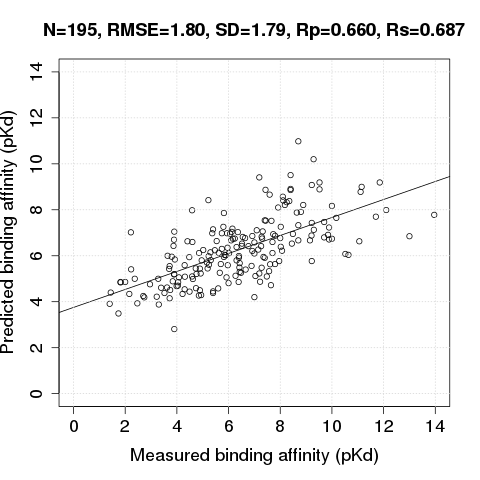
\includegraphics[width=1.4\linewidth,natwidth=480,natheight=480]{../rfcyscore/x4/mlr/trn-247-tst-195-yp.png}
\endminipage\hfill
\minipage{0.5\textwidth}
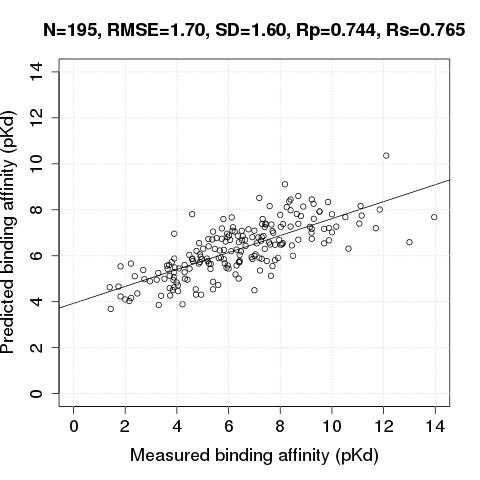
\includegraphics[width=1.4\linewidth,natwidth=480,natheight=480]{../rfcyscore/x46/rf/trn-2280-tst-195-yp.png}
\endminipage\hfill
\caption{MLR::Cyscore (left plot) and RF::CyscoreVinaElem (right plot) performance on PDBbind v2007 core set (N=195).}
\label{fig:tst195}
\end{figure}

\begin{figure}
\minipage{0.5\textwidth}
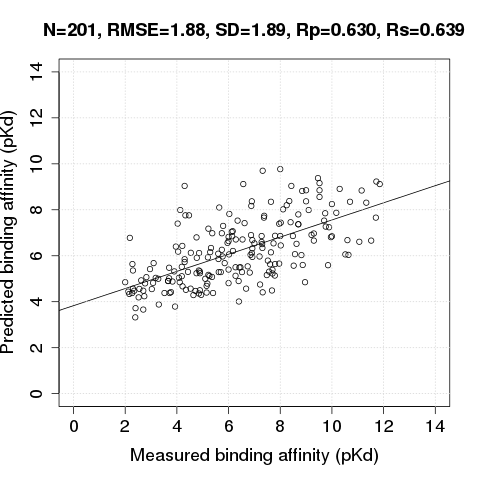
\includegraphics[width=1.4\linewidth,natwidth=480,natheight=480]{../rfcyscore/x4/mlr/trn-247-tst-201-yp.png}
\endminipage\hfill
\minipage{0.5\textwidth}
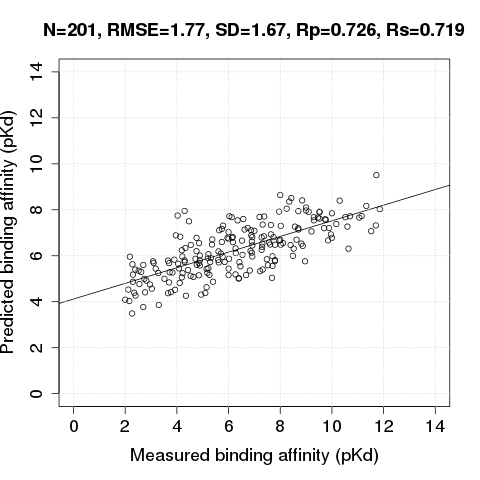
\includegraphics[width=1.4\linewidth,natwidth=480,natheight=480]{../rfcyscore/x46/rf/trn-2280-tst-201-yp.png}
\endminipage\hfill
\caption{MLR::Cyscore (left plot) and RF::CyscoreVinaElem (right plot) performance on PDBbind v2012 core set (N=201).}
\label{fig:tst201}
\end{figure}

\subsection{RF-based scoring functions can be as interpretable as classical ones}

variable importance plot

\subsection{Machine-learning scoring functions assimilate data better than empirical scoring functions}

not only the difference in performance is substantial but grows as more data is available for training, thus increasing the importance of using RF.

\subsection{Cyscore feature usefulness}

Compare x42 and x46

\section{Conclusions}

Machine-learning scoring functions are fundamentally different from classical ones because of not imposing a functional form on the relationship between structural and binding data.

The superior performance of machine-learning scoring functions comes exclusively from the avoidance of the assumed functional form of classical scoring functions. By fixing the same features, training set and test set, any performance difference must necessarily come from the choice of regression model. Moreover, in this case the used training data and features are identical, so will be the domain of applicability of the resulting scoring functions. 

by analysing how their performances improve with the increase of structural and binding data used for training. improvements with data set size can only be gain with the appropriate regression model anyway.

MLR requires meaningful features. RF can benefit from more numerical features.

%%%%%%%%%%%%%%%%%%%%%%%%%%%%%%%%%%%%%%%%%%%%%%%%%%%%%%%%%%%%%%%%%%%%%
%% The "Acknowledgement" section can be given in all manuscript
%% classes.  This should be given within the "acknowledgement"
%% environment, which will make the correct section or running title.
%%%%%%%%%%%%%%%%%%%%%%%%%%%%%%%%%%%%%%%%%%%%%%%%%%%%%%%%%%%%%%%%%%%%%
\begin{acknowledgement}

We gratefully acknowledge the Direct Grant from the Chinese University of Hong Kong, the GRF Grant (Project No. 2150764) from the Research Grants Council of Hong Kong SAR, and the Medical Research Council for a Methodology Research Fellowship (Grant No. G0902106, awarded to P.J.B.). We thank Yang Cao for helping us to reproduce the Cyscore results.

\end{acknowledgement}

%%%%%%%%%%%%%%%%%%%%%%%%%%%%%%%%%%%%%%%%%%%%%%%%%%%%%%%%%%%%%%%%%%%%%
%% The same is true for Supporting Information, which should use the
%% suppinfo environment.
%%%%%%%%%%%%%%%%%%%%%%%%%%%%%%%%%%%%%%%%%%%%%%%%%%%%%%%%%%%%%%%%%%%%%
\begin{suppinfo}



\end{suppinfo}

%%%%%%%%%%%%%%%%%%%%%%%%%%%%%%%%%%%%%%%%%%%%%%%%%%%%%%%%%%%%%%%%%%%%%
%% The appropriate \bibliography command should be placed here.
%% Notice that the class file automatically sets \bibliographystyle
%% and also names the section correctly.
%%%%%%%%%%%%%%%%%%%%%%%%%%%%%%%%%%%%%%%%%%%%%%%%%%%%%%%%%%%%%%%%%%%%%
\bibliography{../refworks}

\end{document}
